\section{Normalization}
Normalization is the process of canonicalizing tokens so that matches occur despite superficial differences in the character sequences of the tokens \cite{Manning2008}. Usual normalization techniques include case folding, lemmatization, stop-word removal, stemming, and so on.

\subsection{Formula Removal}
\label{subsec:formula_rm}
For a technical domain like DSP, there can be many formulas in the text. Formula is a mathematical relationship or rule expressed in symbols. As users would not search for documents based on formulas, those formulas should be removed before indexing documents.

Figure \ref{fig:fm_example} demonstrates an example of original PDF text, converted raw text, and the text after removing formulas. As seen, after converting to raw text from PDF, the formulas become human-unreadable and have no useful meaning. A program\footnote{This program was developed by the undergraduate student Wu Zhenghao.} was thus developed to detect such formulas and replace them with the placeholder \texttt{[FORMULA]}.

\begin{figure}[!htb]
\centering
  \begin{subfigure}{.9\textwidth}
  \centering
  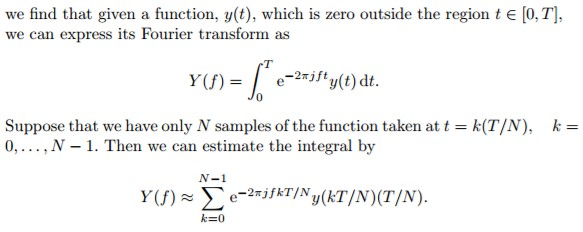
\includegraphics[width=\linewidth]{proposed_methodology_and_system_specifications/sample_pdf.jpg}
  \caption{Sample PDF}
  \label{fig:sfig:pdf}
  \end{subfigure}
  
  \begin{subfigure}{.9\textwidth}
  \centering
  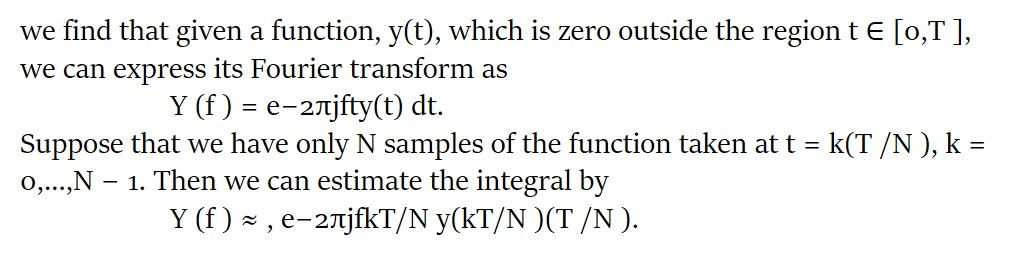
\includegraphics[width=\linewidth]{proposed_methodology_and_system_specifications/sample_raw_text.jpg}
  \caption{Sample Raw Text}
  \label{fig:sfig:raw_text}
  \end{subfigure}
  
  \begin{subfigure}{.9\textwidth}
  \centering
  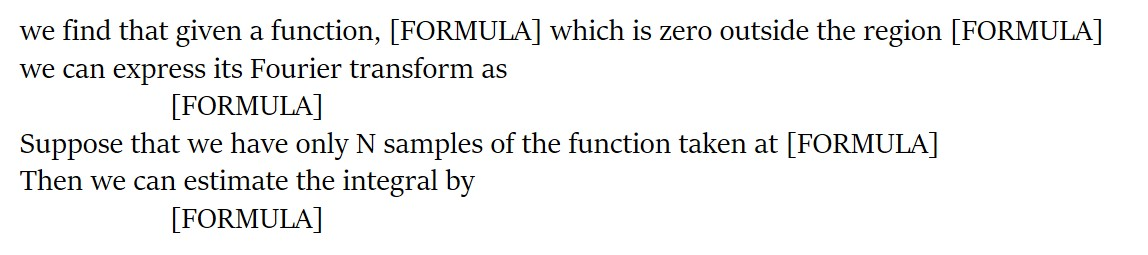
\includegraphics[width=\linewidth]{proposed_methodology_and_system_specifications/sample_normalized_text.jpg}
  \caption{Sample Text after Formula Removal}
  \label{fig:sfig:fm_text}
  \end{subfigure}
 
\caption{Formula Removal Example}
\label{fig:fm_example}
\end{figure}

Dictionary lookup is the approach used to detect formulas and replace them with a placeholder. As shown in Figure \ref{fig:dict_lookup}, a document is first tokenized. Each token is an instance of a sequence of characters in some particular document that are grouped together as a useful semantic unit for processing \cite{Manning2008}. Token preprocessing involves converting a token from upper case to lower case, reducing it to base form, and replacing hyphen with space. The dictionary is a text file with over 354,000 words. A token is flagged as \enquote{formula} if it is neither a number nor a word found in the dictionary after preprocessing. Consecutive placeholders or placeholders separated with punctuations are then merged into one by the program developed. For details on the source code, readers may access the GitHub repository \url{https://github.com/axawzh/TextCleaner}.

\begin{figure}[!htbp]
  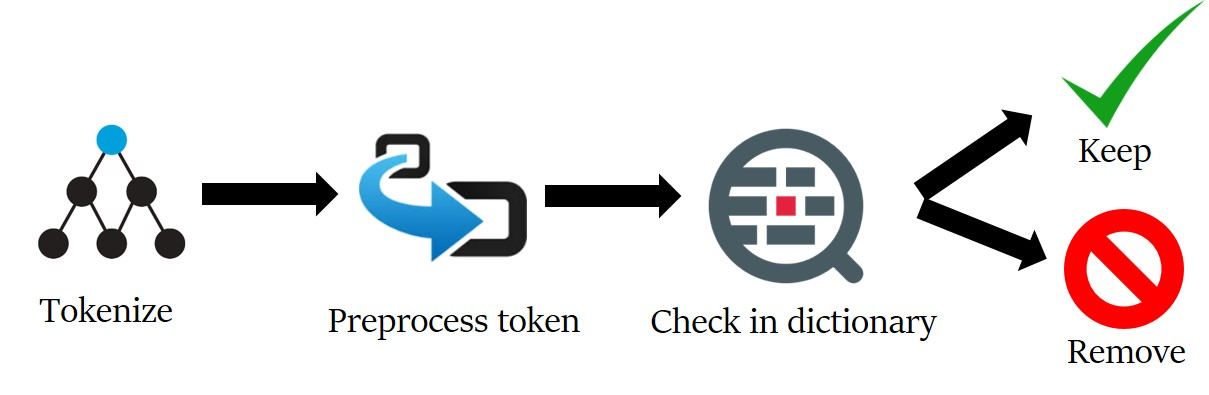
\includegraphics[width=.9\textwidth]{proposed_methodology_and_system_specifications/dictionary_lookup.jpg}
  \caption{Dictionary Lookup}
  \label{fig:dict_lookup}
\end{figure}

The other approach, using regular expressions to detect formulas, was abandoned because it is difficult to maintain a complicated set of regular expressions that can map to a universal set of formulas in a domain. The approach using regular expressions tends to be error-prone and not extensive.

\subsection{Solr Filters}
\label{subsec:solr_filters}
Apache Solr is an open-source Java search engine used for this project. It has built in with some filters for traditional normalization techniques, including stop-word removal, case folding, and stemming. 

\texttt{schema.xml} is a XML configuration file for Solr. It contains all of the details about which fields documents can contain, and what filters to apply when adding documents to the index, or when querying those fields.

In addition to formula removal, mentioned in Section \ref{subsec:formula_rm}, there are 5 filters applied to documents during normalization - \textit{Stop Filter}, \textit{Lower Case Filter}, \textit{English Possessive Filter}, \textit{Keyword Marker Filter}, and \textit{Porter Stem Filter}. An additional filter - \textit{Synonym Filter} is applied to query. The functions of each filter are described in Table \ref{tbl:solr_filters}.

\begin{table}[!htbp]
\centering
\begingroup
\renewcommand{\arraystretch}{1.2}
\caption{Solr Filters}
\label{tbl:solr_filters}
\begin{tabular}{l p{8cm}}
\toprule
\multicolumn{1}{c}{\textbf{Filter}} & \multicolumn{1}{c}{\textbf{Description}} \\ \midrule
Stop Filter & Discards or stops analysis of tokens that are on the given stop words list, named \texttt{stopwords.txt}. \\ \hline
Lower Case Filter & Converts any upper-case letters in a token to the equivalent lower-case token. \\ \hline
English Possessive Filter & Removes possessives (e.g. trailing 's) from words. \\ \hline
Keyword Marker Filter & Protects words in the protected word list from being modified by stemmers. \\ \hline
Porter Stem Filter & Applies the Porter Stemming Algorithm for English. \\ \hline
Synonym Filter & Looks up the token in the list of synonyms and if a match is found, the synonym is emitted in place of the token. 
\\ \bottomrule
\end{tabular}
\endgroup
\end{table}

All these filters are applied before Solr does document indexing. They are configured in \texttt{schema.xml}, which can be found in Solr's installation directory.





